\documentclass[xcolor=svgnames]{beamer}
\mode<presentation>
\usetheme{JuanLesPins}
\usecolortheme[named=Teal]{structure}
\setbeamerfont{structure}{shape=\itshape}

\hypersetup{pdfpagemode=FullScreen} % makes your presentation go automatically to full screen

\setbeamertemplate{background canvas}[vertical
shading][bottom=White!40,top=white!30]
\beamertemplatetransparentcovereddynamicmedium
\useoutertheme{infolines}
%\usepackage{beamerthemesplit}
\usepackage{beamerinnerthemerounded}
\usepackage{beamerouterthemesmoothbars}
\usepackage{subfigure}
\usepackage{multicol}
\usepackage{physics}
\usepackage{amsmath,array}
\usepackage{epsfig}
\usepackage{graphicx}
\usepackage{url}
\usepackage{multimedia}
\usepackage{hyperref}
\usepackage{fancybox}
\usepackage{epstopdf}

\definecolor{lg}{rgb}{0.36,0.99,0.82}
\definecolor{dblue}{rgb}{0,0,.5}
\definecolor{dpink}{cmyk}{.2,1,.1,.04}
\definecolor{purple}{rgb}{0.35,0.04,0.64}
\definecolor{borange}{rgb}{1, .388, 0}
\definecolor{dpurple}{rgb}{0.61,0.22,1.00}
\definecolor{purp}{rgb}{0.44,0.00,0.87}
\definecolor{green}{rgb}{0.00,0.44,0.00}

\newtheorem{theo}{Theorem}
\newtheorem{exa}{Example}
\newtheorem{rem}{Remark}

\def\be{\begin{eqnarray}}%%
\def\ee{\end{eqnarray}}%%
\def\ben{\begin{eqnarray*}}%%
\def\een{\end{eqnarray*}}%%
\def\benum{\begin{enumerate}}%%
\def\eenum{\end{enumerate}}%%
\def\cc#1{\{#1\}}
\def\pp#1{\|#1\|}
\def\ld{\lambda}
\def\l{\leqq}
\def\le{\leqslant}
\def\leq{\leqslant}
\def\geq{\geqslant}
\def\ge{\geqslant}
\def\la{\langle}
\def\ra{\rangle}
\def\Strl{\mathop{\rm Strl}}
\def\eps{\epsilon}
\def\vep{\varepsilon}
\def\rint{\mathop{\rm int}}
\def\bx{\bar{x}}
\def\sx{{x^{\star}}}
\def\bR{\bar{R}}
\def\vsi{\varsigma}
\def\rmint{{\rm int}\,}
\def\ds{\displaystyle}
\newcommand{\norm}[1]{\left\Vert#1\right\Vert}
\newcommand{\tens}[1]{
  \mathbin{\mathop{\otimes}\limits_{#1}}}
\linespread{1.1}
\let\conjugatet\overline

\def\CC{\mathbb{C}}
\def\RR{\mathbb{R}}
\def\MM{\mathbb{M}}
\def\NN{\mathbb{N}}
\def\calL{\mathcal{L}}
\def\calM{\mathcal{M}}
\def\rmint{{\rm int\,}}
\def\cT{\mathcal{T}}
\def\cL{\mathcal{L}}
\def\tau{\cT}
\def\Cl{{cl}\,}
\def\rmint{{\rm int}\,}
\def\disp{\displaystyle}

%***********************************************************
\newcommand{\lr}{\left(}
\newcommand{\rr}{\right)}
\newcommand{\lek}{\left[}
\newcommand{\rek}{\right]}
\newcommand{\lge}{\left\{ }
\newcommand{\rge}{\right\} }
\newcommand{\lb}{\left| }
\newcommand{\rb}{\right| }
\newcommand{\lbl}{\left| }
\newcommand{\rbl}{\right| }
%\newcommand{\ra}{\rangle }
%\newcommand{\la}{\langle }
\newcommand{\es}{\emptyset}
\newcommand{\fa}{\forall}
%\newcommand{\ld}{\lambda}
\newcommand{\real}{\mathbb{R}}
%\newcommand{\norm}[1]{\left\Vert#1\right\Vert}
%\newcommand{\eps}{\epsilon}
\newcommand{\del}{\partial}
\newcommand{\seq}[1]{\left<#1\right>}
%\newtheorem{theorem}{\Large{Theorem}}
\newtheorem{deff}{\Large{Definition}}
\newtheorem{proposition}{\bf Proposition}
%\newtheorem{lemma}{\bf Lemma}
%\newtheorem{example}{\bf Example}
%\newcommand{\lr}{\longrightarrow}
\newcommand{\Ll}{\longleftarrow}
%\newcommand{\ra}{\rightarrow}
%\newcommand{\la}{\leftarrow}
\newcommand{\Lra}{\Leftrightarrow}
\newcommand{\da}{\downarrow}
%\newcommand{\del}{\partial}
\newcommand{\ol}{\overline}
\newcommand{\ul}{\underline}
%\newcommand{\ds}{\displaystyle}
%\newcommand{\fa}{\forall}
\newcommand{\nn}{\nonumber}
\newcommand{\nd}{\noindent}
\newcommand{\imply}{\Rightarrow}
\newcommand{\R}{\mathbb{R}}
\newcommand{\N}{\mathbb{N}}
\newcommand{\h}{\mathbb{H}}
\newcommand{\Z}{\mathbb{Z}}
\newcommand{\B}{\mathcal{B}}
\def\CC{\mathbb{C}}
\def\RR{\mathbb{R}}
\def\MM{\mathbb{M}}
\def\NN{\mathbb{N}}
\def\calL{\mathcal{L}}
\def\calM{\mathcal{M}}
\def\rmint{{\rm int\,}}
\def\cT{\mathcal{T}}
\def\cL{\mathcal{L}}
\def\tau{\cT}
\def\Cl{{cl}\,}
\def\rmint{{\rm int}\,}
\def\disp{\displaystyle}
\def\ds{\displaystyle}
\def\bR{\bar{R}}
%***********************************************************


\title{Quantum Walks on Infinite and Finite Graphs }

\author[MTP Presentation]{MTP Presentation\\[0.5em]
{\scriptsize{By}}\\
[0.5em] Mukesh Bhati \\
(2013MT60604)\\
[0.5em]
{\scriptsize{Under the Supervision of }}\\
[0.5em] Prof. Shravan Kumar\\[2em]}


\institute[] {\scriptsize{Indian Institute of Technology\\  Delhi \\
[0.7em] }}

\date[February 22, 2018]{}
\begin{document}
\frame{\titlepage}


\begin{frame}
\frametitle{Outline of the presentation}
\textbf{Quantum walks on Infinite Graphs}\\
\begin{itemsize}
\begin{enumerate}
    \item On Line.
    \item On 2-D lattice.
\end{enumerate}
\end{itemsize}
\textbf{Quantum walks on Finite Graphs}\\
\begin{itemsize}
\begin{enumerate}
    \item On Cycle.
    \item On 2-D finite lattice.
\end{enumerate}
\end{itemsize}
\end{frame}

\begin{frame}{Quantum walks on Infinite Graphs }
\textbf{Line}
\begin{enumerate}
    \item State Space is Hilbert space. $$H_m \tens{} H_p$$ where $H_p$ is with basis states $\{\ket{n} : n \in \mathbb{Z}\}$ and $H_m$ is $\{\ket{0},\ket{1}\}$
    
\end{enumerate}
    
\end{frame}

\begin{frame}{Quantum walks on Infinite Graphs }
\textbf{Line}
\begin{enumerate}
    \item Shift Operator
    $$ S = \sum_{s=0}^{1}\sum_{n = -\infty}^{\infty} \ket{s,n+(-1)^s}\bra{s,n}$$
    \item Evolution Operator $$ U = S(H \tens{} I)$$
\end{enumerate}
\end{frame}

\begin{frame}{Quantum walks on Infinite Graphs }
\textbf{Line}
\begin{enumerate}
    \item Generic state of the walker
    $$ \ket{\psi(t)} = \sum_{s=0}^{1}\sum_{n = -\infty}^{\infty} \psi_{s,n}(t)\ket{s,n}$$
    \item Probability distribution $$ p_{n}(t) = \abs{\psi_{0,n}(t)}^2 + \abs{\psi_{1,n}(t)}^2$$
\end{enumerate}
\end{frame}

\begin{frame}{Quantum walks on Infinite Graphs}
\textbf{Line}
\begin{enumerate}
    \item Hadamard Operator $$H = \frac{1}{\sqrt{2}}\begin{bmatrix}
                                    1 & 1\\
                                    1 & -1
                                    \end{bmatrix}$$
    \item After applying evolution operator we obtain
    \begin{figure}
    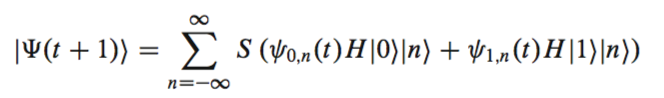
\includegraphics[width = 8cm]{shift.png}
    \end{figure}
    \begin{figure}
        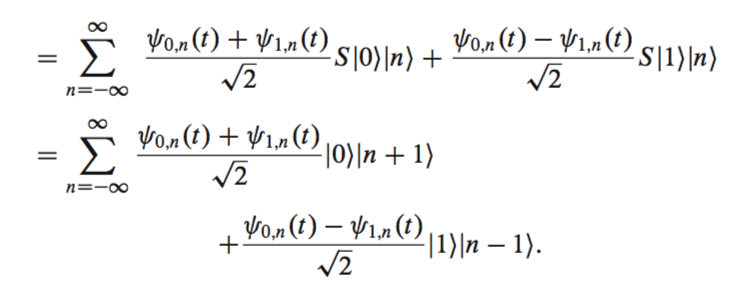
\includegraphics[width = 8cm]{shift2.png}
    \end{figure}
\end{enumerate}
\end{frame}

\begin{frame}{Quantum walks on Infinite Graphs}
\begin{enumerate}
    \item evolution equations
     $$\psi_{0,n}(t+1) = \dfrac{\psi_{0,n-1}(t) + \psi_{1,n-1}(t)}{\sqrt{2}}$$
    $$\psi_{1,n}(t+1) = \dfrac{\psi_{0,n+1}(t) - \psi_{1,n+1}(t)}{\sqrt{2}}$$
\end{enumerate}
\end{frame}

\begin{frame}{Quantum walks on Infinite Graphs}
\begin{figure}
    \centering
    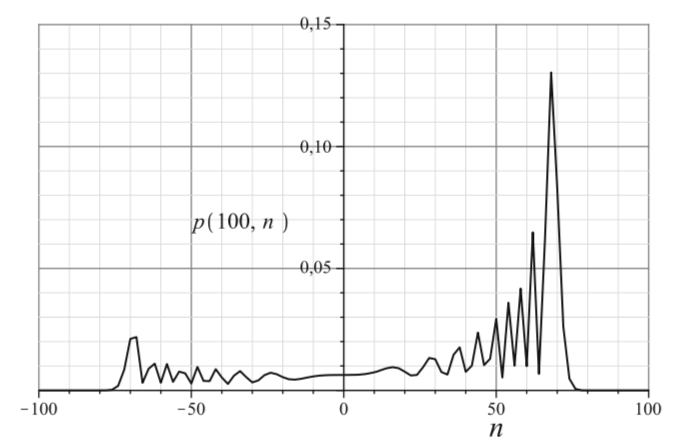
\includegraphics[width = 8cm]{Line_Graph.png}
    \caption{Probability distribution after 100 steps of a quantum walk with the Hadamard coin starting from the initial condition $\ket{\psi(0)} = \ket{0}\ket{n=0}$}
\end{figure}
    
\end{frame}

\begin{frame}{Quantum walks on Infinite Graphs}
\textbf{Analytic Solution}
\begin{enumerate}
    \item \textbf{Fourier Transformation :} The Fourier transformation of a discrete function $ f : \mathbb{Z} \rightarrow \mathbb{C}$ is a continuous function $\hat{f}: [-\pi,\pi] \rightarrow \mathbb{C}$ defined by
    \begin{figure}
        \centering
        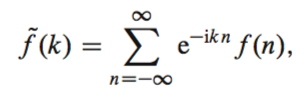
\includegraphics[width = 4cm]{FF.png}
    \end{figure}       
    \begin{figure}
        \centering
        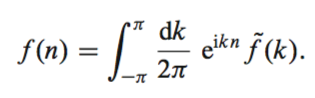
\includegraphics[width = 4cm]{IF.png}
    \end{figure}
\end{enumerate}
\end{frame}

\begin{frame}{Quantum walks on Infinite Graphs}
\begin{enumerate}
    \item $H_p$ basis tramsformation $$\ket{k_k} = \sum_{n=-\infty}^{\infty} e^{ikn}\ket{n}$$
    where $\{\ket{k_k} : -\pi \leq k \leq \pi\}$ called Fourier basis.
\end{enumerate}
\end{frame}

\begin{frame}{Quantum walks on Infinite Graphs}
\begin{enumerate}
    \item Fourier transformation of coefficients
    \begin{figure}
        \centering
        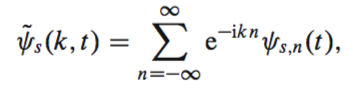
\includegraphics[width = 4.5cm]{CF.png}
    \end{figure}
    \item State of Quantum walk
    \begin{figure}
        \centering
        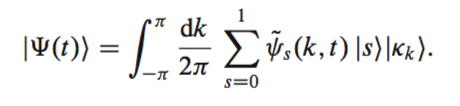
\includegraphics[width = 6cm]{ST.png}
    \end{figure}
\end{enumerate}
\end{frame}

\begin{frame}{Quantum walks on Infinite Graphs}
\begin{enumerate}
    \item Shift Operator on Fourier basis
    \begin{figure}
        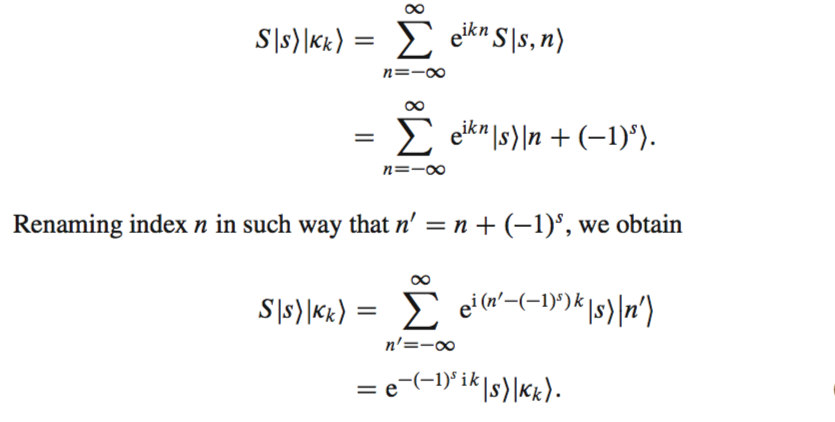
\includegraphics[width = 11cm]{ShiftLine2.png}
    \end{figure}
\end{enumerate}
    
\end{frame}
\begin{frame}{Quantum walks on Infinite Graphs}
    \begin{figure}
    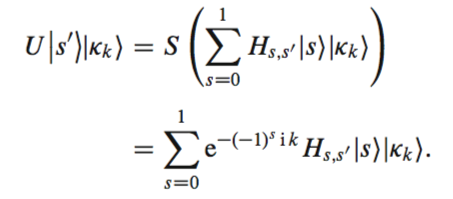
\includegraphics[width = 6cm]{UonLine.png}
    \end{figure}
    \begin{figure}
    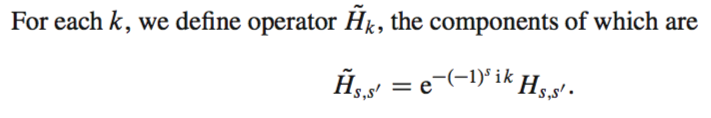
\includegraphics[width = 10cm]{H_K.png}
    \end{figure}
\end{frame}

\begin{frame}{Quantum walks on Infinite Graphs}
In the Matrix Form we have
\begin{figure}
    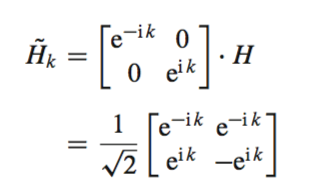
\includegraphics[width = 5cm]{H_k_Matrix.png}
\end{figure}
Diagonalize operator
    \begin{figure}
        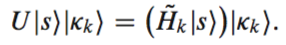
\includegraphics[width = 5cm]{eigen.png}
    \end{figure}
     \begin{figure}
        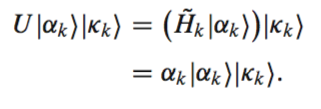
\includegraphics[width = 5cm]{eigen2.png}
    \end{figure}
\end{frame}

\begin{frame}{Quantum walks on Infinite Graphs}
\begin{figure}
    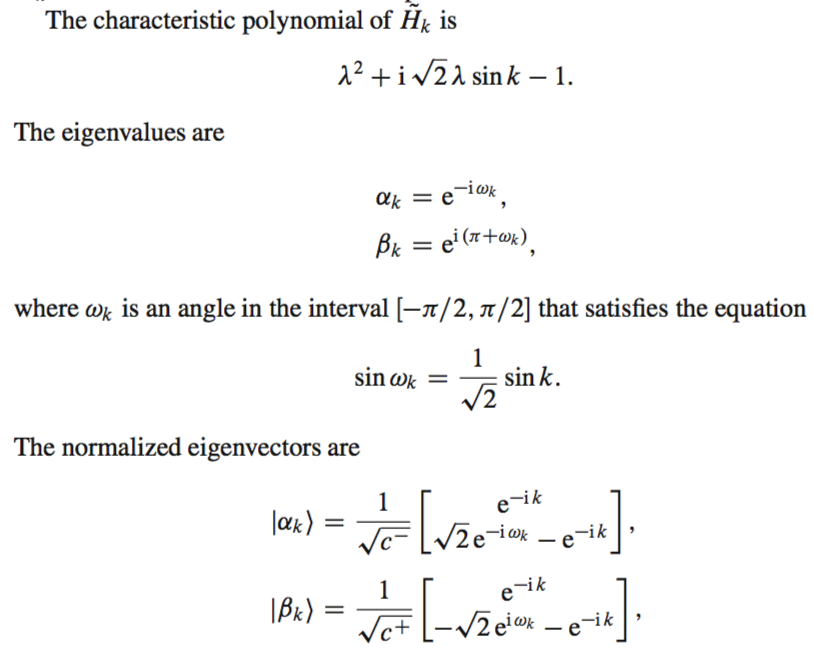
\includegraphics[width = 9cm]{eigen3.png}
\end{figure}
    
\end{frame}

\begin{frame}{Quantum walks on Infinite Graphs}
\begin{figure}
    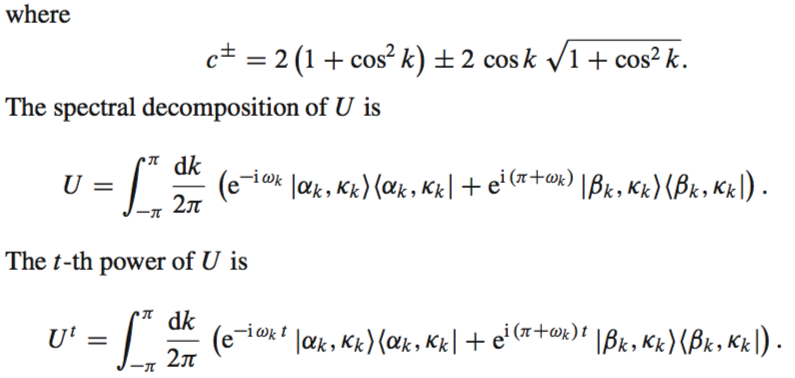
\includegraphics[width = 10cm]{spectral.png}
\end{figure}
    
\end{frame}

\begin{frame}{Quantum walks on Infinite Graphs}
\textbf{Analytical Solution}
\begin{enumerate}
    \item Initial State :
        $ \ket{\psi(0)} = \ket{0}\ket{n=0}$
    \item $\ket{\psi(t)} = U^{t}\ket{\psi(0)} $
\end{enumerate}
    
\end{frame}

\begin{frame}{Quantum walks on Infinite Graphs}
\begin{figure}
    \centering
    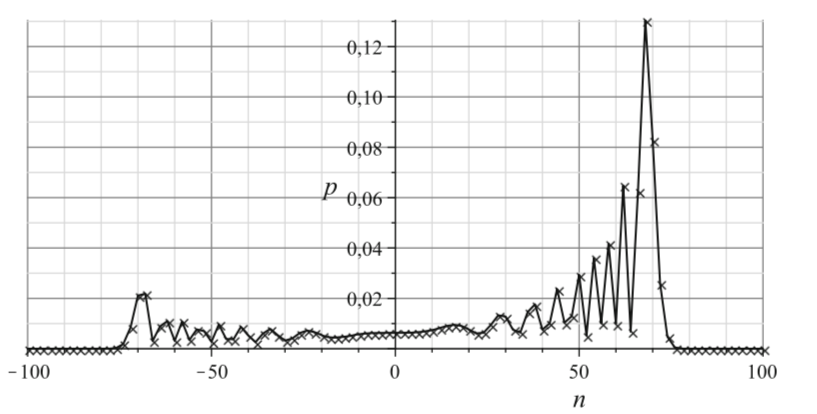
\includegraphics[width = 10cm]{PD_line.png}
    \caption{Probability distribution of the quantum walk on the line after 100 steps from the analytical expression. The cross-shaped points correspond to integer values of n}
\end{figure}
    
\end{frame}

\begin{frame}{Quantum walks on Infinite Graphs}
\textbf{Other Coins : }
Generic Form
\begin{figure}
    \centering
    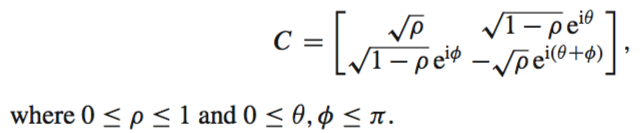
\includegraphics[width = 10cm]{Coin.png}
\end{figure}
\begin{figure}
    \centering
    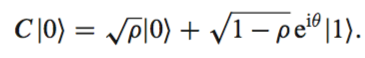
\includegraphics[width = 5cm]{Coin2.png}
\end{figure}
    
\end{frame}

\begin{frame}{Quantum walks on Infinite Graphs}
\textbf{ Two- Dimensional Lattices}
\begin{enumerate}
    \item Hilbert space $H_p$ with computational basis $\{\ket{x,y} : x,y \in \mathbb{Z \}}$
    \item Coin Space $H_m$ with computational basis $\{\ket{i_x,i_y} : 0 \leq i_x,i_y \leq 1 \}$
    \item $H = H_m \tens{}  H_p$
\end{enumerate}
    
\end{frame}

\begin{frame}{Quantum walks on Infinite Graphs}
\textbf{ Two- Dimensional Lattices}
\begin{enumerate}
    \item Generic State
    $$ \ket{\psi(t)} = \sum_{i_x,i_y=0}^{1}\sum_{n = -\infty}^{\infty} \psi_{i_x,i_y;x,y}(t)\ket{i_x,i_y}\ket{x,y}$$
    \item Shift Operator
            $$S\ket{i_x,i_y}\ket{x,y} = \ket{i_x,i_y}\ket{x+(-1)^{i_x},y+(-1)^{i_y}}$$
    
\end{enumerate}
    
\end{frame}

\begin{frame}{Quantum walks on Infinite Graphs}
\textbf{ The Hadamard Coin}
\begin{enumerate}
    \item $C = H \tens{} H$
    $$C = \frac{1}{2}\begin{bmatrix}
                                1 & 1 & 1 & 1\\
                                    1 & -1 & 1 & -1\\
                                    1 & 1 & -1 & -1\\
                                    1 & -1 & -1 & 1
                                    \end{bmatrix}$$
    \item Initial State : $\ket{\psi(0)} = \dfrac{\ket{0}+i\ket{1}}{\sqrt{2}} \tens{} \dfrac{\ket{0} +i\ket{1}}{\sqrt{2}} \tens{} \ket{x=0,y=0}$
    
\end{enumerate}
    
\end{frame}

\begin{frame}{Quantum walks on Infinite Graphs}
\begin{figure}
    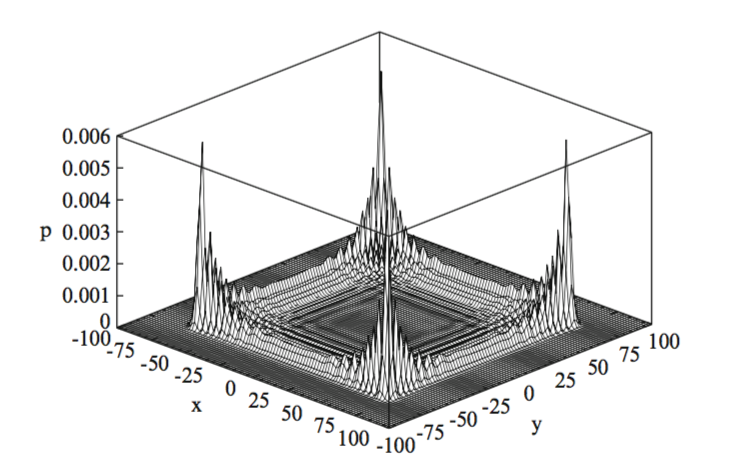
\includegraphics[width = 9cm]{Hadamard2D.png}
    \caption{Probability distribution of the quantum walk in the two-dimensional lattice with the Hadamard coin after 100 steps}
\end{figure}
    
\end{frame}

\begin{frame}{Quantum walks on Infinite Graphs}
\textbf{ The Fourier Coin}
\begin{enumerate}
    \item
    $$C = \frac{1}{2}\begin{bmatrix}
                                1 & 1 & 1 & 1\\
                                    1 & -i & 1 & -i\\
                                    1 & -1 & 1 & -1\\
                                    1 & -i & -1 & i
                                    \end{bmatrix}$$
    \item Initial State : $\ket{\psi(0)} =\dfrac{1}{2}(\ket{00} + \dfrac{1-i\ket{01}}{\sqrt{2}} + \ket{10} - \dfrac{1-i\ket{11}}{\sqrt{2}})\ket{x=0,y=0}$
    
\end{enumerate}
    
\end{frame}

\begin{frame}{Quantum walks on Infinite Graphs}
\begin{figure}
    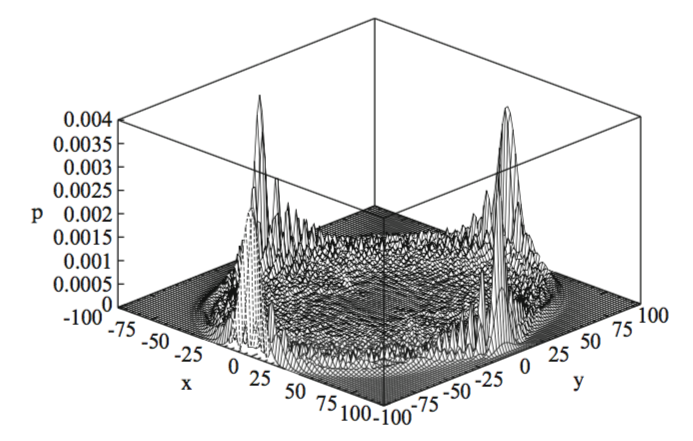
\includegraphics[width = 9cm]{Fourier2D.png}
    \caption{Probability distribution of the quantum walk in the two-dimensional lattice with the Fourier coin after 100 steps}
\end{figure}
    
\end{frame}

\begin{frame}{Quantum walks on Finite Graphs }
\textbf{Cycle}
\begin{enumerate}
    \item State Space is Hilbert space. $$H^2 \tens{} H^N$$ where $H^N$ is with basis states $\{\ket{j} : 0\leq j \leq N-1 \}$ and $H^2$ is $\{\ket{0},\ket{1}\}$
    
\end{enumerate}
    
\end{frame}

\begin{frame}{Quantum walks on Finite Graphs }
\textbf{Cycle}
\begin{enumerate}
    \item Shift Operator
    $$ S = \sum_{s=0}^{1}\sum_{n = 0}^{N-1} \ket{s,j+(-1)^s}\bra{s,j}$$
    \item Evolution Operator $$ U = S(H \tens{} I)$$
\end{enumerate}
\end{frame}

\begin{frame}{Quantum walks on Finite Graphs }
\textbf{Line}
\begin{enumerate}
    \item Generic state of the walker
    $$ \ket{\psi(t)} = \sum_{s=0}^{1}\sum_{n = 0}^{N-1} \psi_{s,n}(t)\ket{s,j}$$
    \item Probability distribution $$ p_{j}(t) = \abs{\psi_{0,j}(t)}^2 + \abs{\psi_{1,j}(t)}^2$$
\end{enumerate}
\end{frame}

\begin{frame}{Quantum walks on Finite Graphs}
\begin{figure}
    \centering
    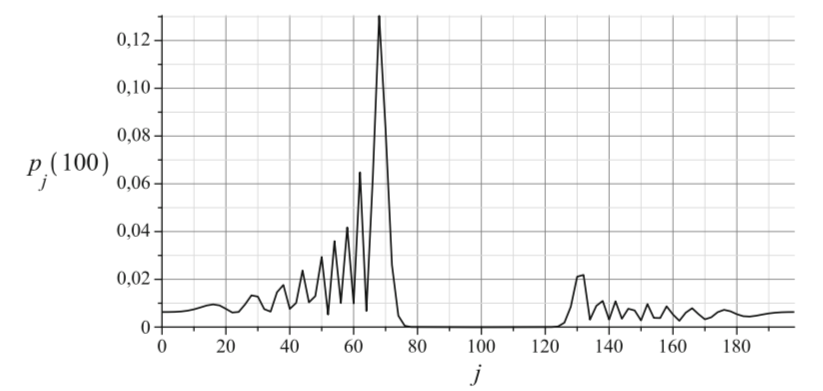
\includegraphics[width = 10cm]{PDFinite.png}
    \caption{Probability distribution of the quantum walk on cycle with N D 200 after 100 steps starting from initial condition $\ket{\psi(0)} = \ket{0}\ket{0}.$}
\end{figure}
\end{frame}

\begin{frame}{References}
\begin{enumerate}
 \item Norio Konno, Philiphe Biane, Quantum Potential Theory, Lecture Notes in Mathematics 2008
 \item J. Kempw. Quantum random walk:an introductory overview. Contemp. Phy. 2003
\item R. Portugal, Quantum walks and search algorithm Springer, 2013
\end{enumerate}
\end{frame}


\end{document}}